\documentclass[11.5pt, twoside, a4paper]{article}
\usepackage{graphicx, amssymb, amsmath, amsthm, xfrac, mathabx, upgreek, fancyhdr, float, underscore, url}
\usepackage[section]{placeins}
\usepackage[]{mcode}

\begin{document}

\title{Intelligent Adaptive Systems: Assignment}
\author{Chanelle Lee}
\date{\today}
\maketitle

\section{Introduction}

\subsection{Adaptive Neuro-Fuzzy Inference System (ANFIS)} %Needs a bit more work
ANFIS is a `fuzzy inference system implemented in the framework of adaptive networks' developed in the early 1990s \cite{JangANFIS}. It is called a hybrid neuro-fuzzy technique as it uses the learning capabilities of neural networks to `tune' the membership functions of a Sugeno-type Fuzzy Inference System. 

\subsection{The Task}
The task of this assignment is to use ANFIS to derive a representation of the inverse kinematics of the Lynxmotion robotic arm. In order to investigate this, Matlab's anfis toolbox will be used, with the main questions to be explored:
\begin{enumerate}
\item What is the ideal density of training data? A balance between efficiency and effectiveness is needed; as the more training data points the more accurate the results, but the longer the system takes.
\item How to generate the initial fuzzy inference system; should genfis1 or genfis2 be used? And what parameters should they take?
\item For how many epochs should ANFIS run?
\item What should be the spread of the training data? Should the training data points be uniform over the workspace or concentrated near singularities?
\end{enumerate}

 Due to time constraints, the simpler problem of a planar RR arm will be used to investigate the first three questions; as the data sets required to train the system are much smaller, and so more exploration of parameter settings of the ANFIS is achievable. Then, the best parameters found will be used to train for a planar RRR arm and as the planar RRR arm gives a representation of the Lynxmotion arm in the XZ-plane, the final question will be investigated. Finally, these findings will be implemented on the Lynxmotion arm and compared against analytical solutions.

\section{Planar RR Arm}

For this section, the Lynxmotion arm will be reduced the to the planar RR problem as described in Fig.\ref{fig:2Link}\footnote{Altered to match findings in Section\ref{sec:elbowIssues}}. The input-output data pairs used to train and validate will be the joint angles $\theta_2$ and $\theta_3$ and their corresponding values in values in the XZ-plane.

\begin{figure} %Might be a bit large
\begin{center}
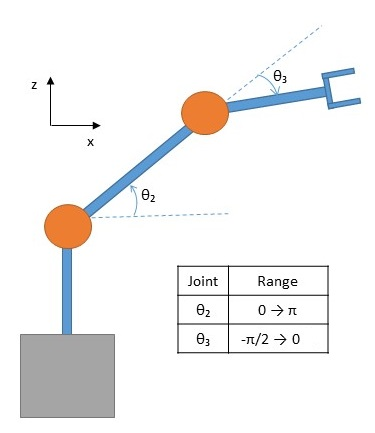
\includegraphics{2Link.jpg}
\caption{Planar RR Robotic Arm \label{fig:2Link}}
\end{center}
\end{figure}

\subsection{Joint Angle Range Issues} \label{sec:elbowIssues}

When the experiments were first run there were very large errors in the Cartesian and joint space (Table.\ref{tab:range})\footnote{Genfis1 with two membership functions, 100 data points and 500 epochs.} and this was discovered to be because the range $\theta_3$ was set to $\left[-\pi/2,\pi/2\right]$, This meant that for each point in Cartesian space there were two possible solutions in the joint space with either a positive or negative value for $\theta_3$. This corresponded to the fact that each point in Cartesian space can be reached by the end effector in one of two configurations; elbow up or elbow down. This was solved by limiting the range of $\theta_3$ to only negative values, i.e. limiting the robotic arm to only elbow down configurations, which is much more realistic in terms of the Lynxmotion arm's capabilities.

\begin{table}
\begin{center}
\scalebox{0.7}{
\begin{tabular}{|c||c|c|c|c|c|c|c|}\hline
$\theta_3$ range & trnRMSE2 & chkRMSE2 & trnRMSE3 & chkRMSE3 & cartRMSE & cartMin & cartMax\\ \hline\hline
$\left[-\pi/2, \pi/2\right]$ & 0.3792 &  0.3794 &   0.7387  &  0.7389 &  35.7034  &  0.0497 &  99.4345\\ \hline
$\left[-\pi/2, 0\right]$ & 0.0312 &   0.0311  &  0.0682 &   0.0687  &  5.5590  &  0.0651  & 111.7742 \\ \hline
\end{tabular}}
\caption{Results from changing range of $\theta_3$. \label{tab:range}}\end{center}
\end{table}


\subsection{Number of Epochs}
The number of epochs controls the length of time ANFIS spends tuning the membership functions of the Fuzzy Inference System (FIS) and setting this is a matter of comparing the accuracy attained against the time taken. In Fig.\ref{fig:2000Epochs}\footnote{Genfis1 with two membership functions and 100 data points} it is clear that if only the first fifty epochs are considered the training and validation errors of the joint angles are still falling and there is little evidence to show how far they might further fall, but when one thousand epochs are run there is clearly little improvement after five hundred epochs. Table.\ref{tab:epochs} also shows that the Root-Mean-Squared-Error (RMSE) in the Cartesian space reduces by less than a tenth of a millimetre from five hundred to one thousand epochs despite it taking twice as long to run. Interestingly, there is also little change in the Cartesian RMSE between one hundred epochs and five hundred epochs. In conclusion, the best number of epochs to use for further experiments is five hundred as confidence can be had that training and validation errors in the joint angles have stabilised by this epoch, but there is little point continuing as neither the error in the joint angles or the Cartesian RMSE appear to decrease enough to be beneficial.

\begin{figure}
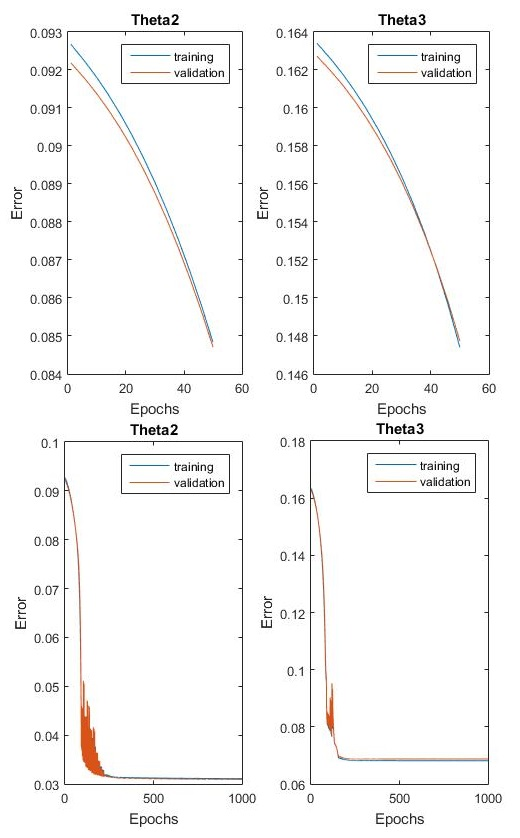
\includegraphics[width=\linewidth]{Epochs.jpg}
\caption{Planar RR Arm with run for 50 and 1000 Epochs\label{fig:2000Epochs}}
\end{figure}

\begin{table} 
\scalebox{0.7}{
\begin{tabular}{|c | c | c | c | c | c | c | c | c | c  | c | } 
\hline
dataPoints & Epochs & MFs & trnRMSE2 & chkRMSE2 & trnRMSE3 & chkRMSE3 & cartRMSE & cartMin & cartMax & time \\ \hline \hline
100 &	50   &	2 &	0.0848 &	0.0847 &	0.1474 &	0.1477 &	8.9448 &	0.0728 &	63.0842  &	2.38 \\ \hline
100 &	100  &	2 &	0.0358 &	0.0356 &	0.0795 &	0.0801 &	5.8968 &	0.0425 &	25.2959  &	4.38 \\ \hline
100 &	500  &	2 &	0.0312 &	0.0311 &	0.0682 &	0.0687 &	5.5590 &	0.0651 &	111.7742 &	20.17 \\ \hline
100 &	1000 &	2 &	0.0311 &	0.0309 &	0.0681 &	0.0687 &	5.5723 &	0.0184 &	111.7176 &	39.92 \\ \hline
\end{tabular}}
\caption{Number of Epochs Experiment \label{tab:epochs}}
\end{table}

\subsection{Optimising Genfis1}
To investigate the best parameters using Genfis1 to create the FIS two loops were used to explore:
\begin{itemize}
\item The number of membership functions between two and ten.
\item The number of data points from ten, twenty, fifty, one hundred, two hundred and five hundred.
\end{itemize}
The results from this can be seen in Appendix 1, Table \ref{tab:2LinkGenfis1}; the last half of the two hundred data

\subsubsection{Number of Membership Functions}
The number of membership functions is used by genfis1 to set the number of membership functions of each variable in the FIS \cite{genfis1}. This is important to explore as more membership functions can lead to an increase in accuracy due to a greater capacity for complexity, much like increasing the degree of a polynomial line of best fit. However, too great a capacity for complexity can lead to over-fitting, where the system has been trained so well on the training data, that it is unable to generalise in the areas in between. To continue the polynomial line of best fit example, this would be analogous to increasing the degree of the line of best fit until it passes through every given data point, but in doing so losing the overall shape of the data being described. In order to check for over-fitting, validation data is used so that the error at points not in the training set can be monitored. Then over-fitting can be identified as where the error at training points drops to near zero, but the error at validation points begins to climb, see Figure.\ref{fig:Overfitting}. A countermeasure against over-fitting is to increase the density of the training data, as seen in Figure.\ref{fig:Genfis1}, where the behaviour with different numbers of membership functions varies greatly with the density of the training data.
\begin{figure}
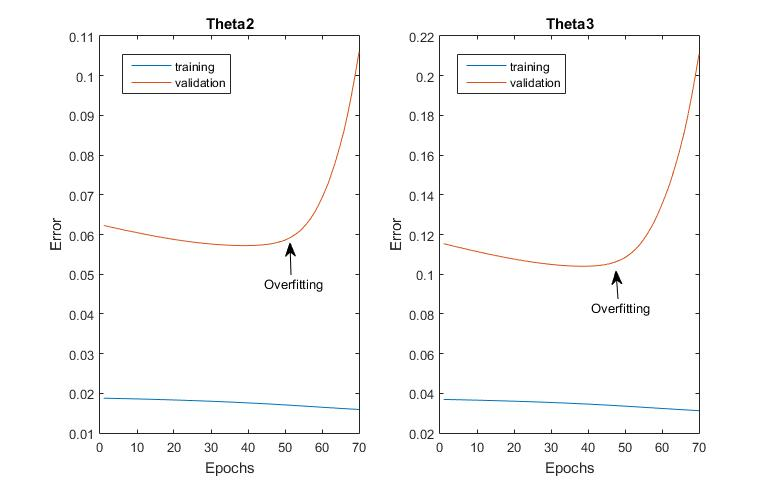
\includegraphics[width=\linewidth]{OverFitting.jpg}
\caption{Example of Over-Fitting\label{fig:Overfitting}}
\end{figure}

Another repercussion of increasing membership functions is that this also increases the time the systems takes to train and so once again a balance needs to be struck between accuracy and efficiency. Considering the results from Table \ref{tab:2LinkGenfis1} and displayed in Figure.\ref{fig:Genfis1}, it is clear that the most choosing the most efficient number of membership functions depends greatly on the density of the training data. Perhaps surprisingly, Table \ref{tab:mfs} shows that, for the training data densities experimented with, two membership functions performed the best in terms of Cartesian RMSE and time. This is mostly likely due to the negative effects of over-fitting at low training data densities.

\begin{table} 
\begin{center}
\begin{tabular}{|c | c | c |} 
\hline
MFs &   Average cartRMSE & Average time \\ \hline \hline
2 & 15.2 &    5.9 \\ \hline
3 & 25.8 &   14.0 \\ \hline
4 & 46.2 &   31.0 \\ \hline
5 & 65.7 &   65.5 \\ \hline
6 & 37.7 &  125.7 \\ \hline
7 & 64.1 &  227.6 \\ \hline
8 & 52.3 &  380.2 \\ \hline
9 & 67.0 &  603.8 \\ \hline
10 & 51.1 & 904.0 \\ \hline
\end{tabular}
\caption{The average Cartesian RMSE and time taken for each number of membership functions from Table \ref{tab:2LinkGenfis1} \label{tab:mfs}}\end{center}
\end{table}

\begin{figure}
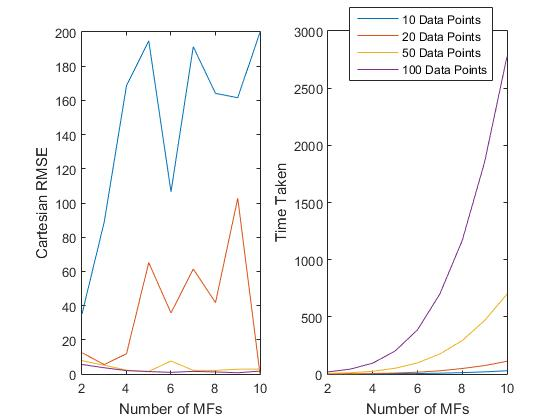
\includegraphics[width=\linewidth]{numMFs.jpg}
\caption{Time and Cartesian RMSE vs Number of Membership Functions for Different Numbers of Data points (from Table \ref{tab:2LinkGenfis1})\label{fig:Genfis1}}
\end{figure}

\subsubsection{Density of Training Data}

A limitation of ANFIS is that it uses supervised learning and as such needs training input-output data, which can be difficult to source for problems and the additional need for validation data only adds to this. Even with a problem such as this task, where finding input-output pairs is relatively easy using the forward kinematic equations, the density of training data is still an issue as it requires more time and computational power to train. On the other hand, the greater the density of the training data, the greater the accuracy due to less speculation needed to fill in the missing areas of information.

As the planar RR problem is being used as a starting point for the planar RRR one, scalability also have to be considered. ANFIS suffers from the curse of dimensionality, in that adding even just one more variable, or dimension, to the problem can cause massive increase in the computing power and time needed to train the FIS. Considering all this and Figure.\ref{fig:Genfis1} having fifty data points appears to be a good trade off between accuracy and time. 

\subsection{Optimising Genfis2} \label{sec:GA}
Genfis2 uses subtractive clustering to generate a Sugeno-type FIS structure \cite{genfis2} and in this experiment a genetic algorithm is used to try and determine optimal radii inputs for each joint. A genetic algorithm was chosen here, over any other type of optimisation algorithm, as it was feared that there would be many local optima, e.g. the optimal radius for each cluster. For the sake of convenience, Matlab's built in ga function was used for this experiment; with hard constraints set on the chromosome. However, as genfis2 only accepts radii to one decimal place and the population the ga produces is to four decimal places, the inputs are rounded before genfis2. As the aim of the genetic algorithm is to find the most efficient set of parameters, as opposed to the most accurate, the original fitness function used to evaluate the performance of the chromosomes is the Cartesian RMSE mitigated by the time taken. Figure.\ref{fig:GA} displays the results\footnote{With fifty data points and five hundred epochs.} from the genetic algorithm and the best chromosome found corresponded to,
\begin{equation*}
\theta_2\text{ radii }= [0.5, 0.8, 0.2] \quad \& \quad \theta_3\text{ radii } = [0.4, 0.7,  0.5], 
\end{equation*}
which has a Cartesian RMSE of 3.35 and took 980 seconds.

Time problems were experienced using the genetic algorithm, as the time taken for each generation is the length of time for fitness function (in this case genfis2 and anfis) to run, multiplied by the population size. As such only a small population size of ten was used for this experiment and as such the genetic algorithm ended after a short number of generations on a result which may not be globally optimal. In terms of practicality, the length of time necessary to compute the fitness function should in future be taken into account when considering the use of a genetic algorithm. Furthermore, the need to round the chromosomes from Matlab's built-in ga function, meant there was a lot of unnecessary variation within the population.

\begin{figure}
\begin{center}
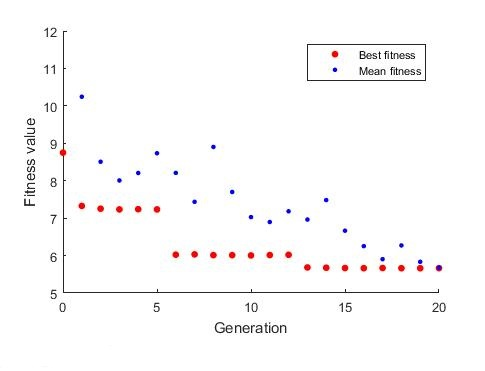
\includegraphics[width=\linewidth]{GAResults.jpg}
\caption{Genetic Algorithm Results for Genfis2 on Planar RR Arm\label{fig:GA}}
\end{center}
\end{figure}

\subsection{Concluding Remarks}
Although genfis1 performed much better for accuracy and time for the planar RR arm, \cite{faq} states that, because genfis1 relies upon grid partitioning it is more susceptible to `the curse of dimensionality'. This suggests that genfis1 would struggle with the planar RRR arm and even more so with the full Lynxmotion Arm. Also, as discussed in Section \ref{sec:GA}, the results of the genetic algorithm were not ideal and so genfis2 could perform much better than witnessed. Thus, genfis2 is the method to be carried forwards to the planar RRR problem. 

\section{Planar RRR Arm}

This section will deal with the planar RRR arm problem as described in Figure.\ref{fig:3Link}. As there is now an additional joint angle to find, a new input variable is needed and this will be the pitch of the arm.
\begin{figure} 
\begin{center}
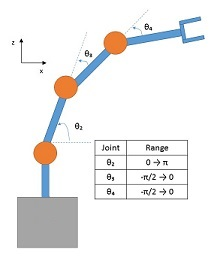
\includegraphics{3Link.jpg}
\caption{Planar RRR Robotic Arm \label{fig:3Link}}
\end{center}
\end{figure}

\subsection{Experiments with Radii Values}
In order to determine suitable radii values for constructing the FIS structure for $\theta_4$, and whether to use the radii values found for $\theta_2$ and $\theta_3$ in Section \ref{sec:GA} the following options were tested:
\begin{enumerate}
\item A control where the radii values were all set to 0.5.
\item A secondary control where the radii values for $\theta_2$ and $\theta_3$ are kept, and for $\theta_4$ are all set to 0.5.
\item Keeping the radii values for $\theta_2$ and $\theta_3$ the same and setting $\theta_4$ as a mix of the two.
\item Keeping the radii values for $\theta_2$, but setting $\theta_4$ to the previous values of $\theta_3$ and $\theta_3$ as a mix of the two. This was based on the thinking that as $\theta_3$ was in fact the new angle to learn, as the planar RR arm had no joint attached to other joints at both ends.
\end{enumerate}
The results of these experiments can be seen in Table \ref{tab:situations} with the radius for the pitch set to the default of 0.5. The best performance was from the third set of radii values, and this is most likely due to the significant decrease in the validation RMSE in $\theta_4$. Although surprisingly this was not the case for the reduction in validation RMSE for $\theta_3$ for the fourth set of radii values.

\begin{table} 
\begin{center}
\begin{tabular}{|c | c | c | c | c| c|} 
\hline
Situation &   cartRMSE & time & chkRMSE2 & chkRMSE3 & chkRMSE4 \\ \hline \hline
1 & 24.09 & 2776 & 0.0731& 0.0661& 0.0353 \\ \hline
2 & 13.00 & 1144 & 0.0451& 0.0781& 0.0353 \\ \hline
3 & 12.65 & 2504 & 0.0442& 0.0750& 0.0283 \\ \hline
4 & 13.02 & 2391 & 0.0442& 0.0603& 0.0416 \\ \hline
\end{tabular}
\caption{Results for Planar RRR Arm in the Four Situations Specified \label{tab:situations}}
\end{center}
\end{table}


\subsection{Spread of Training Data} \label{sec:spread}

So far the data points for training and validation have been sampled uniformly across the ranges of the joint angles; however, if the sampling of the data points was concentrated more heavily in the areas producing the most errors, the accuracy could be increased. The first step is to identify the regions in the joint space causing the greatest errors in the Cartesian space. From Figure.\ref{fig:carterrors}, these are identified as;
\begin{itemize}
\item $\theta_2 = \pi$, 
\item $\theta_3 = 0$, $\theta_3=\frac{-pi}{2}$, and, 
\item $\theta_4 = 0$.
\end{itemize}

Unfortunately, as can be seen in Figure.\ref{fig:spread} the accuracy did not improve and did in fact worsen; in the regions with the concentrated sampling the errors do improve, but in the sparser regions the errors grew. Although disappointing, this is believed to be due the already sparseness of the data points and essentially there not being enough to favour any region and it not seriously hamper the effectiveness in another.

\begin{figure}
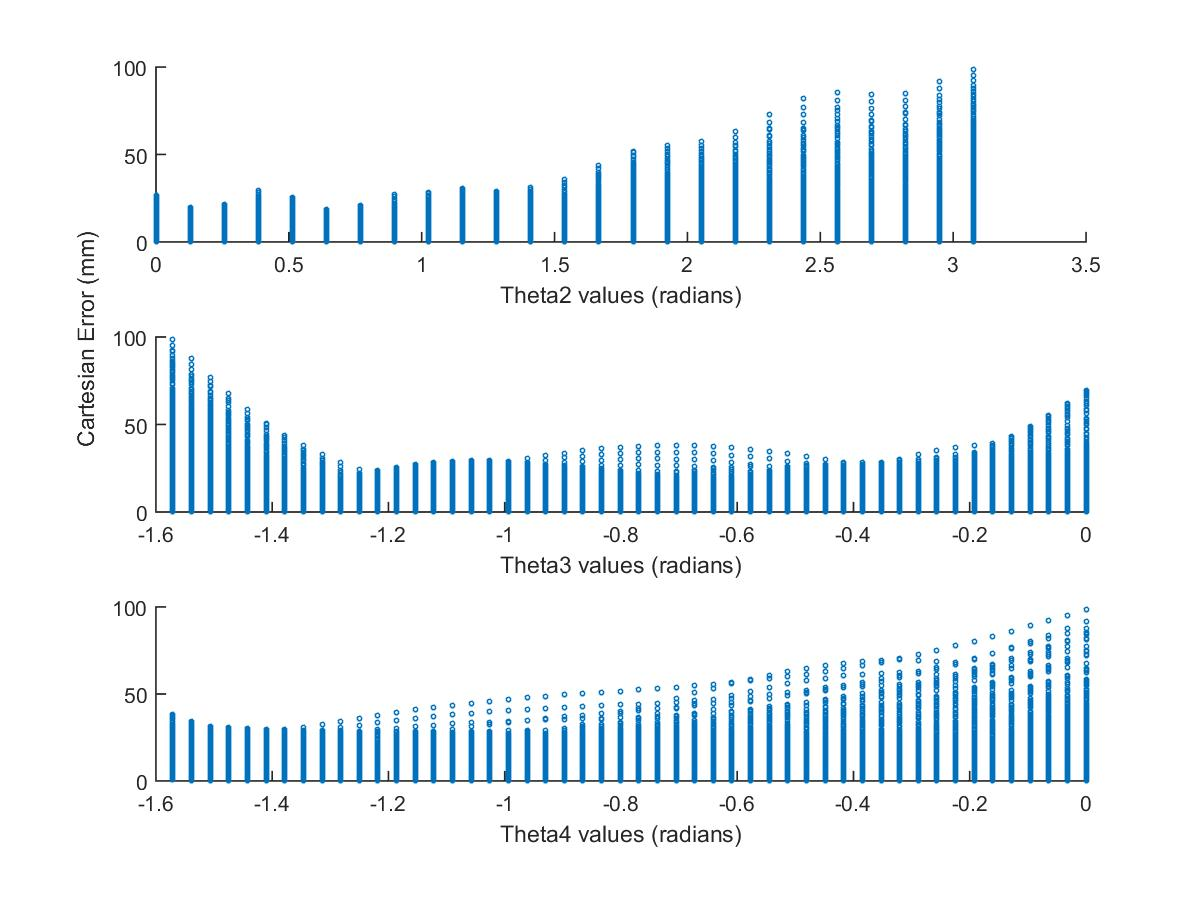
\includegraphics[width=\linewidth]{cartesianerrorsTHETA.jpg}
\caption{Cartesian RMSE in Joint Space\label{fig:carterrors}}
\end{figure}

\begin{figure}
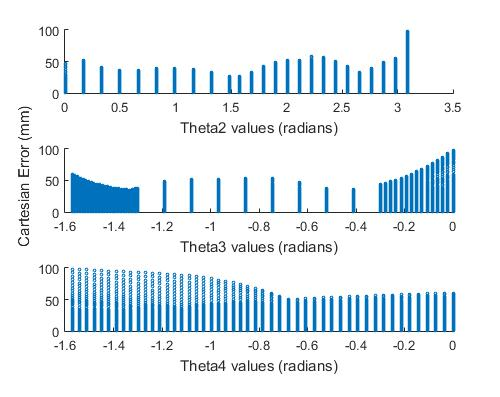
\includegraphics[width=\linewidth]{spreadChange.jpg}
\caption{Cartesian RMSE in Joint Space after Change of Spread\label{fig:spread}}
\end{figure}

\subsection{Changing Joint Angle Ranges}

Another method to reduce the Cartesian RMSE is to either remove the singularities identified in Section \ref{sec:spread} or possibly, where they present a boundary to the region, extend the region beyond them in the hopes that performing training either side will reduce the overall error. Figure.\ref{fig:rangereduce} shows the results of cropping the singularities from the joint space, but, although this method achieved a much better Cartesian RMSE of 4.38mm, it has not truly solved the issue of these troublesome regions, just ignored them. It is a worthy method to consider though, as if the robot arm only needs a limited workspace, then training across singularities when it is unnecessary is pointless. 

\begin{figure}
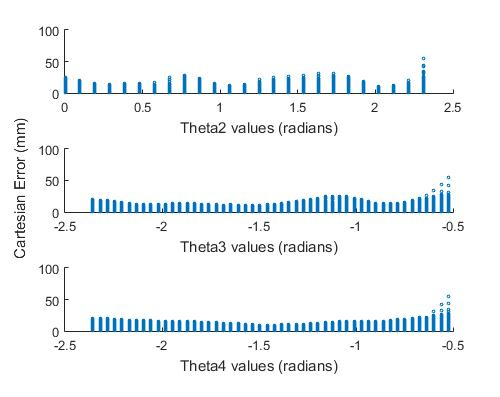
\includegraphics[width=\linewidth]{ReducedRanges.jpg}
\caption{Cartesian RMSE in Joint Space after Reducing Joint Space Ranges\label{fig:rangereduce}}
\end{figure}

\section{Lynxmotion Arm}

In order to turn the planar RRR arm to a representation of the Lynxmotion robotic arm another variable $\theta_1$, the rotation around the z-axis, is needed. As $\theta_1$ only affects behaviour on the XY-plane it is unnecessary to train it upon Z and the pitch and similarly, there is no need to train $\theta_2$, $\theta_3$ or $\theta_4$ on Y. As such the  Limiting the input for the training of each angle to only what is necessary could help mitigate the scalability issues caused by the additional dimension. Unfortunately, keeping a training data density of fifty data points proved infeasible in the time frame and so this was reduced to just twenty data points.

A control run setting all the radii values to the default resulted in a disappointing Cartesian RMSE of 436.2mm with some errors reaching 800mm, with the validation error for $\theta_2$, $\theta_3$ and $\theta_4$ a magnitude higher than for the planar RRR arm. This is most likely due to the reduction in training data density. For the final run with the radii values for $\theta_1$ set to the default 0.5 and those for the other angles the same as for the planar RRR arm, the Cartesian RMSE error was 436.17mm and once again the validation RMSE is a magnitude higher than for the planar RRR arm.

Considering the membership functions of the FIS before and after training, it is disappointing to see that there is little change apart from for $\theta_4$, implying that little training actually occurred. This is perhaps due to the low density of the training data.
\begin{figure}
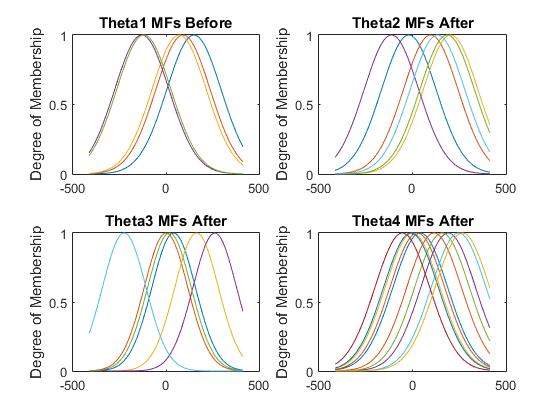
\includegraphics[width=\linewidth]{MFsBefore.jpg}
\caption{Membership Functions Before Training \label{fig:MFsBefore}}
\end{figure}

\begin{figure}
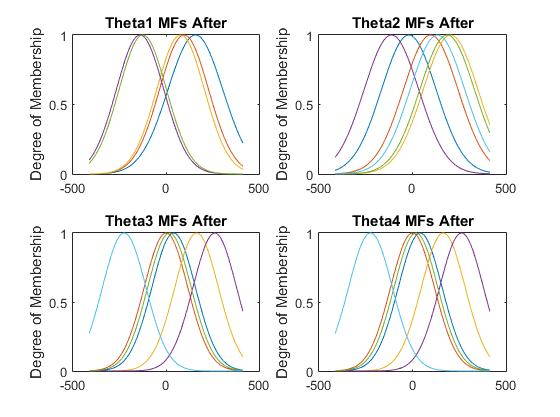
\includegraphics[width=\linewidth]{MFsAfter.jpg}
\caption{Membership Functions After Training \label{fig:MFsAfter}}
\end{figure}



\section{Conclusion}
In conclusion, this report has explored the task of using ANFIS to calculate the inverse kinematics of the Lynxmotion Arm. Although the accuracy of the final method used is not idea, it is felt that, if the available time had been used more wisely to fully explore all the methods mentioned in the report, far better results could have been obtained.


\section{Appendix 1 - Experiment Results}

\begin{table} 
\scalebox{0.7}{
\begin{tabular}{|c | c | c | c | c | c | c | c | c | c  | c | } 
\hline
dataPoints & Epochs & MFs & trnRMSE2 & chkRMSE2 & trnRMSE3 & chkRMSE3 & cartRMSE & cartMin & cartMax & time \\ \hline \hline
10 &	500 &	2 &	0.0441 &	0.1769 &	0.0595 &	0.2102 &	35.0791 &	2.3860 &	151.5126 &		0.32 \\ \hline
10 &	500 &	3 &	0.0075 &	0.6026 &	0.0186 &	1.5039 &	88.9466 &	1.7816 &	300.7353 &		0.44 \\ \hline
10 &	500 &	4 &	0.0016 &	1.5343 &	0.0029 &	2.8815 &	168.6123 &	3.1412 &	464.0428 &		0.99 \\ \hline
10 &	500 &	5 &	0.0005 &	2.3307 &	0.0001 &	1.6801 &	194.8358 &	8.2084 &	519.1364 &		2.03 \\ \hline
10 &	500 &	6 &	0.0000 &	0.7692 &	0.0000 &	1.1000 &	106.5546 &	1.1282 &	342.4532 &		3.91 \\ \hline
10 &	500 &	7 &	0.0000 &	1.0441 &	0.0000 &	1.5253 &	191.3857 &	6.1158 &	625.5818 &		7.09 \\ \hline
10 &	500 &	8 &	0.0000 &	0.8198 &	0.0000 &	0.5227 &	164.0823 &	2.6072 &	624.2153 &		11.81 \\ \hline
10 &	500 &	9 &	0.0000 &	0.8749 &	0.0000 &	0.7083 &	161.5942 &	7.4095 &	629.0190 &		18.56 \\ \hline
10 &	500 &	10 &	0.0000 &	1.0498 &	0.0000 &	0.7715 &	199.8085 &	4.0177 &	629.9484 &		28.28 \\ \hline
20 &	500 &	2 &	0.0487 &	0.0707 &	0.0747 &	0.1185 &	12.4193 &	0.4108 &	103.9274 &		0.74 \\ \hline
20 &	500 &	3 &	0.0196 &	0.0490 &	0.0395 &	0.0945 &	5.5069 &	0.3025 &	24.1058 &		1.74 \\ \hline
20 &	500 &	4 &	0.0204 &	0.0871 &	0.0407 &	0.1851 &	11.8301 &	0.1035 &	64.8913 &		3.95 \\ \hline
20 &	500 &	5 &	0.0083 &	1.0060 &	0.0151 &	1.4404 &	65.1519 &	0.4279 &	462.7651 &		8.43 \\ \hline
20 &	500 &	6 &	0.0037 &	0.1839 &	0.0074 &	0.3333 &	35.6708 &	0.2279 &	256.3560 &		15.52 \\ \hline
20 &	500 &	7 &	0.0018 &	0.3554 &	0.0035 &	0.5666 &	61.4179 &	0.3654 &	572.2944 &		28.16 \\ \hline
20 &	500 &	8 &	0.0013 &	0.2046 &	0.0025 &	0.3664 &	41.7306 &	0.2340 &	212.7630 &		48.13 \\ \hline
20 &	500 &	9 &	0.0011 &	0.3528 &	0.0015 &	0.3827 &	102.7713 &	0.4082 &	488.5110 &		73.61 \\ \hline
20 &	500 &	10 &	0.0007 &	0.3804 &	0.0015 &	0.6136 &	109.5996 &	1.7098 &	521.3018 &		111.39 \\ \hline
50 &	500 &	2 &	0.0371 &	0.0362 &	0.0694 &	0.0769 &	7.7817 &	0.1222 &	98.5986 &		4.46 \\ \hline
50 &	500 &	3 &	0.0248 &	0.0250 &	0.0451 &	0.0512 &	5.1415 &	0.1326 &	99.1554 &		10.80 \\ \hline
50 &	500 &	4 &	0.0206 &	0.0221 &	0.0411 &	0.0435 &	2.2461 &	0.0248 &	13.0735 &		23.72 \\ \hline
50 &	500 &	5 &	0.0164 &	0.0177 &	0.0326 &	0.0348 &	1.5393 &	0.0175 &	7.7383 &		50.42 \\ \hline
50 &	500 &	6 &	0.0124 &	0.0572 &	0.0253 &	0.0767 &	7.5921 &	0.0401 &	209.7884 &		96.92 \\ \hline
50 &	500 &	7 &	0.0112 &	0.0242 &	0.0220 &	0.0487 &	2.1075 &	0.0208 &	23.5713 &		175.22 \\ \hline
50 &	500 &	8 &	0.0103 &	0.0217 &	0.0195 &	0.0383 &	2.1102 &	0.0155 &	22.4959 &		292.86 \\ \hline
50 &	500 &	9 &	0.0087 &	0.0214 &	0.0171 &	0.0451 &	2.8006 &	0.0122 &	26.8913 &		468.32 \\ \hline
50 &	500 &	10 &	0.0081 &	0.0197 &	0.0159 &	0.0394 &	2.8987 &	0.0078 &	45.3157 &		699.17 \\ \hline
100 &	500 &	2 &	0.0312 &	0.0311 &	0.0682 &	0.0687 &	5.5590 &	0.0651 &	111.7742 &		18.10 \\ \hline
100 &	500 &	3 &	0.0236 &	0.0235 &	0.0446 &	0.0458 &	3.6464 &	0.0521 &	29.4106 &		42.97 \\ \hline
100 &	500 &	4 &	0.0200 &	0.0202 &	0.0396 &	0.0400 &	1.9688 &	0.0156 &	10.9047 &		95.06 \\ \hline
100 &	500 &	5 &	0.0158 &	0.0160 &	0.0314 &	0.0318 &	1.4229 &	0.0046 &	14.1410 &		201.28 \\ \hline
100 &	500 &	6 &	0.0117 &	0.0132 &	0.0230 &	0.0261 &	0.9550 &	0.0016 &	8.5618 &		386.25 \\ \hline
100 &	500 &	7 &	0.0105 &	0.0116 &	0.0199 &	0.0211 &	1.5349 &	0.0052 &	19.1859 &		700.12 \\ \hline
100 &	500 &	8 &	0.0100 &	0.0107 &	0.0196 &	0.0212 &	1.1876 &	0.0100 &	35.0601 &		1167.94 \\ \hline
100 &	500 &	9 &	0.0084 &	0.0096 &	0.0163 &	0.0189 &	0.7292 &	0.0023 &	7.2050 &		1854.52 \\ \hline
100 &	500 &	10 &	0.0077 &	0.0107 &	0.0152 &	0.0205 &	1.7005 &	0.0072 &	49.1822 &		2776.96 \\ \hline
200 &	500 &	2 &	0.0300 &	0.0301 &	0.0672 &	0.0675 &	5.6355 &	0.0679 &	168.8529 &		76.53 \\ \hline
200 &	500 &	3 &	0.0236 &	0.0235 &	0.0440 &	0.0441 &	3.2618 &	0.0141 &	21.6430 &		175.64 \\ \hline
200 &	500 &	4 &	0.0197 &	0.0197 &	0.0387 &	0.0388 &	1.8952 &	0.0042 &	11.8753 &		387.51 \\ \hline
200 &	500 &	5 &	0.0146 &	0.0146 &	0.0295 &	0.0295 &	1.6488 &	0.0123 &	8.9011 &		816.60 \\ \hline
200 &	500 &	6 &	0.0114 &	0.0115 &	0.0224 &	0.0226 &	0.8359 &	0.0016 &	6.2123 &		1554.44 \\ \hline
\end{tabular}}
\caption{Planar RR Arm - Genfis1 Parameter Experiment \label{tab:2LinkGenfis1}}
\end{table}

\section{Appendix 2 - Matlab Code}

\lstinputlisting{AnfisFullArm.m}
\lstinputlisting{ThreeArmGenfis2.m}
\lstinputlisting{TwoArmGenfis1.m}
\lstinputlisting{TwoArmGenfis2.m}
\lstinputlisting{TwoArmGenfis2GA.m}

\bibliographystyle{unsrt}
\bibliography{IAS}{}


\end{document}